\mode<presentation>
{
  \usetheme{CambridgeUS}
  \usecolortheme{whale}
  \usecolortheme{lily}

  \setbeamercovered{transparent}
  \usefonttheme[onlymath]{serif}
}

\title[\BodePlotsIShortName] % (optional, use only with long paper titles)
{\course: \BodePlotsIName\license}

\subtitle
{Lecture \BodePlotsINumber} % (optional)



% Delete this, if you do not want the table of contents to pop up at
% the beginning of each subsection:
%\AtBeginSection[]
%{
%  \begin{frame}<beamer>{Outline}
%    \tableofcontents[currentsection,currentsubsection]
%  \end{frame}
%}


% If you wish to uncover everything in a step-wise fashion, uncomment
% the following command:

%\beamerdefaultoverlayspecification{<+->}


\begin{document}

\begin{frame}
  \titlepage
\end{frame}

\mode<article>{
\maketitle
\tableofcontents
}

%\mode<presentation>{
%\begin{frame}{Outline}
%  \tableofcontents
%  % You might wish to add the option [pausesections]
%\end{frame}}

\section{Re-Cap}

In the previous lecture, we found

\begin{itemize}
\item For a stable linear system, if the input is a sinusoid, then at steady state, the output is a sinusoid
\item The sinusoidal steady state response is completely determined by
\[
|G(j\omega)|\mbox{ and }\angle G(j\omega).
\]
Specifically, if
\[
u(t) = A\cos(\omega t + \theta)
\]
then
\[
y_{ss}(t) = |G(j\omega)|A\cos(\omega t + \theta  + \angle G(j\omega))
\]
\item $G(j\omega)$ is called the {\em frequency response function}
\item A generic first order system without a zero has a transfer function of the form
\[
G(s) = K\frac{\sigma}{s+\sigma}
\]
We plug in $j\omega$ to find the frequency response function, which is
\[
G(j\omega) = K\frac{\sigma}{j\omega + \sigma} = K\frac{1}{\frac{j\omega}{\sigma} +1}.
\]
\item 
The magnitude of the frequency response function is
\begin{align*}
|G(j\omega)| &= \left|K\frac{1}{\frac{j\omega}{\sigma} +1}\right|\\
 &= |K|\frac{|1|}{\left|j\frac{\omega}{\sigma} +1\right|}\\
 &= K\frac{1}{\sqrt{1 + \left(\frac{\omega}{\sigma}\right)^{2}}}
\end{align*}
\item The phase of the frequency response is
\begin{align*}
\angle G(j\omega) & = \angle  K\frac{1}{\frac{j\omega}{\sigma} +1}\\
& = \angle K + \angle 1 - \angle \left(\frac{j\omega}{\sigma}+1\right) \\
& = 0 + 0 - \tan^{-1}\left(\frac{\omega}{\sigma}\right)\\
& = -\tan^{-1}\left(\frac{\omega}{\sigma}\right)
\end{align*}

\end{itemize}

\section{Frequency Response for a  First Order System}
We want to plot how the magnitude and phase of the frequency response function changes as $\omega$ changes. The first thing we note is that in these expressions, $\omega$ is always divided by $\sigma$. Thus, what will be important is the relative size of $\omega$ with respect to $\sigma$. In the following table, we plug in some different values for $\omega/\sigma$.

\begin{frame}{Magnitude Table}
\begin{center}
\begin{tabular}{cccc}
\toprule
\multirow{2}{*}{$\frac{\omega}{\sigma}$} & \multirow{2}{*}{$\frac{K}{\sqrt{\left(\frac{\omega}{\sigma}\right)^{2}+1}}$} & \multicolumn{2}{c}{$-\tan^{-1}\left(\frac{\omega}{\sigma}\right)$} \\
& & radians & degrees\\\midrule
\rule{0pt}{12pt}.01 & $K$ & -0.01 & -0.58$^{\circ}$\\
\rule{0pt}{16pt}0.1 & $\frac{K}{1.005}$ & -0.0997 & -5.7$^{\circ}$ \\
\rule{0pt}{16pt}1 & $\frac{K}{\sqrt{2}}$ & -0.785 & -45$^{\circ}$\\
\rule{0pt}{16pt}10 & $\frac{K}{10.05}$ & $-1.47$ & $-84.3^{\circ}$\\
\rule{0pt}{16pt}100 & $\frac{K}{100}$ & $-1.56$ & $-89.4^{\circ}$\vspace{4pt}\\\bottomrule
\end{tabular}
\end{center}
\end{frame}

To visualize this data, we will plot the magnitude and phase vs frequency. However, we will utilize a log scale for frequency as well as re-scale the magnitude in decibels.

\begin{definition}
Given system frequency response, $G(j\omega)$ the magnitude response in decibels (dB) is
\[
L_{\mbox{dB}}=20 \log_{10}\left(|G(j\omega)|\right)
\]
\qed
\end{definition}

Using the data for the table above, and recalling that $\log_{10}(ab) = \log_{10}(a)+\log_{10}(b)$, we can re-calculate the magnitude in decibels

\begin{center}
\begin{tabular}{ccc}
\toprule
$\frac{\omega}{\sigma}$ & $\frac{K}{\sqrt{\left(\frac{\omega}{\sigma}\right)^{2}+1}}$ & magnitude in dB \\\midrule
\rule{0pt}{12pt}.01 & $K$ & $20\log_{10}(K)$ \\
\rule{0pt}{16pt}0.1 & $\frac{K}{1.005}$ & $20\log_{10}(K)-.04$ \\
\rule{0pt}{16pt}1 & $\frac{K}{\sqrt{2}}$ &  $20\log_{10}(K)-3$ \\
\rule{0pt}{16pt}10 & $\frac{K}{10.05}$ &  $20\log_{10}(K)-20$\\
\rule{0pt}{16pt}100 & $\frac{K}{100}$ &  $20\log_{10}(K)-40$ \\\bottomrule
\end{tabular}
\end{center}

We will plot the magnitude in decibels vs. frequency on a log scale. A log scale is created by plotting the point $x$ at a distance $\log_{10}(x)$ from the origin.  An example of a log plot with some selected points is shown below, along with the related linear scale. 

\begin{frame}{Log scale}
\begin{center}
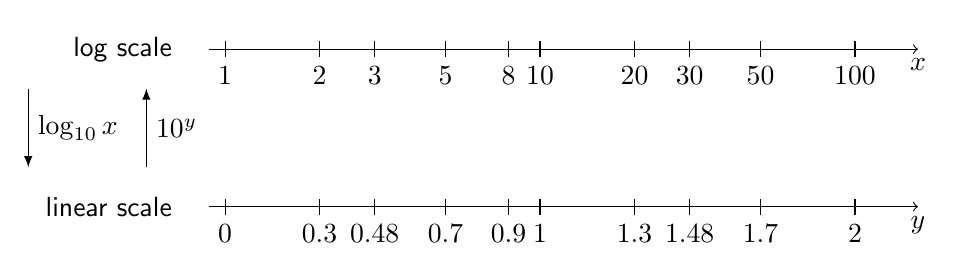
\begin{tikzpicture}
%\draw (0,0) node {\includegraphics[width=4in,bb= 0 0 432 50,clip]{figures/logscaleplot}};
\draw[->] (-.2,0) node[left=10pt] {\textsf{log scale}} -- ++(9,0) node[below] {$x$}; 
\draw[-] (0,0) ++(0,.1) -- ++(0,-.2) node[below] {$1$};
\draw[-] (1.2,0) ++(0,.1) -- ++(0,-.2) node[below] {$2$};
\draw[-] (1.9,0) ++(0,.1) -- ++(0,-.2) node[below] {$3$};
\draw[-] (2.8,0) ++(0,.1) -- ++(0,-.2) node[below] {$5$};
\draw[-] (3.6,0) ++(0,.1) -- ++(0,-.2) node[below] {$8$};
\draw[-] (4,0) ++(0,.1) -- ++(0,-.2) node[below] {$10$};
\draw[-] (4+1.2,0) ++(0,.1) -- ++(0,-.2) node[below] {$20$};
\draw[-] (4+1.9,0) ++(0,.1) -- ++(0,-.2) node[below] {$30$};
\draw[-] (4+2.8,0) ++(0,.1) -- ++(0,-.2) node[below] {$50$};
\draw[-] (8,0) ++(0,.1) -- ++(0,-.2) node[below] {$100$};
\draw[->] (-.2,-2) node[left=10pt] {\textsf{linear scale}} -- ++(9,0) node[below] {$y$}; 
\draw[-] (0,-2) ++(0,.1) -- ++(0,-.2) node[below] {$0$};
\draw[-] (1.2,-2) ++(0,.1) -- ++(0,-.2) node[below] {$0.3$};
\draw[-] (1.9,-2) ++(0,.1) -- ++(0,-.2) node[below] {$0.48$};
\draw[-] (2.8,-2) ++(0,.1) -- ++(0,-.2) node[below] {$0.7$};
\draw[-] (3.6,-2) ++(0,.1) -- ++(0,-.2) node[below] {$0.9$};
\draw[-] (4,-2) ++(0,.1) -- ++(0,-.2) node[below] {$1$};
\draw[-] (4+1.2,-2) ++(0,.1) -- ++(0,-.2) node[below] {$1.3$};
\draw[-] (4+1.9,-2) ++(0,.1) -- ++(0,-.2) node[below] {$1.48$};
\draw[-] (4+2.8,-2) ++(0,.1) -- ++(0,-.2) node[below] {$1.7$};
\draw[-] (8,-2) ++(0,.1) -- ++(0,-.2) node[below] {$2$};
\draw[->,>=latex] (-1,-1.5) -- node[pos=.5,right] {$10^{y}$}  ++(0,1);
\draw[->,>=latex] (-2.5,-0.5) -- node[pos=.5,right] {$\log_{10}x$}  ++(0,-1);
\end{tikzpicture}
\end{center}
\end{frame}


Note that equidistant points are related by a common multiplicative factor, rather than additive factor as is the case in a linear scale. Thus, if we measure the distance from 1 to 10, we see that it is the same distance from 2 to 20 or 10 to 100, since each of these numbers are related by a factor of 10. A factor of 10 in a log scale is called a {\em decade}.

\begin{frame}{Plot with log-scale on x-axis}
\begin{center}
\begin{tikzpicture}
\draw[very thick,<->,>=|] (-3.8,2.5) -- node[pos=.5,above=0pt] {\small \textsf{one decade} } ++(2.7,0); 
\draw[very thick,<->,>=|] (-3.0,3.1) -- node[pos=.5,above=0pt] {\small \textsf{one decade} } ++(2.7,0); 
\draw[very thick,<->,>=|] (1.46,2.5) -- node[pos=.5,above=0pt] {\small \textsf{one decade} } ++(2.7,0); 
\draw (0,0) node {\includegraphics[width=4in]{figures/logscaleplot}};
\end{tikzpicture}
\end{center}
\end{frame}

The plot of magnitude in decibels vs. frequency in log scale then looks like the following.

\begin{frame}{Magnitude Bode plot}
\begin{center}
\begin{tikzpicture}
\draw (0,0) node {\includegraphics[width=4in]{figures/bodeplot}};
\draw (-5.5,.5) node[rotate=90] {\large \textsf{Magnitude (dB)}};
\end{tikzpicture}
\end{center}
\end{frame}

The plot of phase in degrees vs. frequency in log scale is 

\begin{frame}{Phase Bode plot}
\begin{center}
\includegraphics[width=4in]{figures/bodeplotphase}
\end{center}
\end{frame}

Both the magnitude and phase bode plots have a lot of structure to them. By breaking them up into different sections, we can come up with ways for easily sketching an approximate Bode plot.

The magnitude response has two main sections - a low frequency part that is flat, and a high frequency part that decreases linearly on the log plot. The frequency that divides these two sections is $\sigma$, the magnitude of the pole. In the following plot, the lines that define the linear approximation are overlaid on the exact Bode plot. Note that the line for $\omega > \sigma$ decreases by $20$ decibels every time the frequency increases by a factor of 10, which is a decade. Thus, the slope of the line is $-20$dB/dec.

\begin{frame}{Linear Approximation for Magnitude Bode plot}
\begin{center}
\begin{tikzpicture}
\draw (0,0) node {\includegraphics[width=4in]{figures/bodeplot}};
\draw (-5.5,.5) node[rotate=90] {\large \textsf{Magnitude (dB)}};
\draw[color=red,line width=3pt] (-3.25,1.975) -- ++(5,0);
\draw[color=red,line width=3pt] (.115,2.5) -- (5.1,-1.2);
\draw(-2,3) node {$\omega< \sigma$};
\draw(3,3) node{$\omega > \sigma$};
\draw(3.2,1.2) node{$-20$\textsf{dB/dec}};
\draw[thick] (2.15,1) -- ++(.2,0) -- ++(0,-.16);
\end{tikzpicture}
\end{center}
\end{frame}


A similar approximation is possible for the phase plot, except in this case there are three regions: $\omega < \frac{\sigma}{10}$, $\frac{\sigma}{10} < \omega < 10\sigma$ and $\omega > 10\sigma$, and the slope of the decreasing line is $-45^{\circ}$/dec.

\begin{frame}{Linear Approximation for Phase Bode plot}
\begin{center}
\begin{tikzpicture}
\draw (0,0) node {\includegraphics[width=4in]{figures/bodeplotphase}};
\draw(-2.5,3) node {$\omega< \frac{\sigma}{10}$};
\draw(.5,3) node{$\frac{\sigma}{10} < \omega < 10\sigma$};
\draw(3.5,3) node{$\omega > 10\sigma$};
\draw[color=red,line width=3pt] (-3.5,2.15) -- ++(2.5,0);
\draw[color=red,line width=3pt] (-1.95,2.5) -- ++(5.1,-3.9);
\draw[color=red,line width=3pt] (2.1,-.98) -- ++(2.5,0);
\draw(1.3,0.9) node{$-45^{\circ}$\textsf{/dec}};
\draw[thick] (.5,.7) -- ++(.2,0) -- ++(0,-.16);
\end{tikzpicture}
\end{center}
\end{frame}

\begin{example}
Using linear approximations, sketch the Bode plot for the transfer function
\[
G(s) = \frac{2}{s+7}.
\]

We note that this system has a pole at $s=-7$, thus $\sigma=7$. To find the DC gain, we divide top and bottom by 7
\[
G(s) = \frac{\frac{2}{7}}{\frac{s}{7}+1}.
\]

The magnitude Bode plot should start at $20\log_{10}(2/7) = -10.9$. The plot will be flat until 7 rad/s, and then decrease at -20 dB/dec.

\begin{frame}{Bode magnitude plot example}
\begin{center}
\begin{tikzpicture}
\draw (0,0) node {\includegraphics[width=4in]{figures/blankbodeplot}};
\draw[color=red,line width=3pt] (-3.5,1.3) -- ++(5.05,0);
\draw[color=red,line width=3pt] (1.55,1.3) -- ++(3.0,-2.05);
\end{tikzpicture}
\end{center}
\end{frame}

The phase Bode plot should be flat one decade before and one decade after 7 rad/s, or  before $7/10=.7$ rad/s and after $7(10)=70$ rad/s. In between, it should drop at $45^{\circ}$/dec.

\begin{frame}{Bode phase plot example}
\begin{center}
\begin{tikzpicture}
\draw (0,0) node {\includegraphics[width=4in]{figures/blankbodeplotphase}};
\draw[color=red,line width=3pt] (-3.5,2.15) -- ++(2.3,0);
\draw[color=red,line width=3pt] (-1.2,2.15) -- (4.3,-.98);
\draw[color=red,line width=3pt] (4.3,-.98) -- ++(.45,0);
\end{tikzpicture}
\end{center}
\end{frame}

\end{example}

\section{Lecture Highlights}
The primary takeaways from this article include
\begin{enumerate}
\setlength{\itemsep}{5pt}
\setlength{\parskip}{0pt}
\setlength{\parsep}{0pt}
\item The sinusoidal steady state magnitude and phase can be evaluated across a range of frequencies and plotted on two log-scale plots; the result is called a \textit{Bode plot}.
\item The Bode plot can be used to quickly evaluate the sinusoidal steady state response of a dynamic system to a sinusoidal input frequency.
\item There are asymptotic rules for sketching Bode plots by hand that depend on the number and locations of poles and zeros; this article gives an example of the rules for $1^{st}$ order systems with left-half plane (LHP) stable poles only.
\end{enumerate}



\section{Quiz Yourself}

\subsection{Questions}

\begin{enumerate}
\setlength{\itemsep}{5pt}
\setlength{\parskip}{0pt}
\setlength{\parsep}{0pt}
\item Using the linear approximation rules, sketch the Bode plot for the transfer function
\[
G(s) = \frac{20}{s+2}
\]
From your sketch, find the magnitude in dB and the phase in degrees for the sinusoidal response at $\omega=5$ rad/s. 
\item Using the linear approximation rules, sketch the Bode plot for the transfer function
\[
G(s)=\frac{3}{s+10}.
\]

\end{enumerate}

\subsection{Solutions}
\begin{enumerate}
\setlength{\itemsep}{5pt}
\setlength{\parskip}{0pt}
\setlength{\parsep}{0pt}
\item \rule{12pt}{0pt}
\begin{center}
\includegraphics[width=5in]{quizfigures/1asoln}\\
\includegraphics[width=5in]{quizfigures/1bsoln}
\end{center}
\item \rule{12pt}{0pt}
\begin{center}
\includegraphics[width=5in]{quizfigures/2asoln}\\
\includegraphics[width=5in]{quizfigures/2bsoln}
\end{center}
\end{enumerate}


\end{document}


